\section{Controller Prefilter}

The step response of the controller exhibited a major problem that when the step was applied, the ball would roll off the wrong side of the track. This can be seen in figure \ref{3:fig:stepresponse} where the purple line (representing the ball position) starts at the initial condition and goes towards the target, but jumps backwards briefly. This is the controller compensating for the fact that the ball is initially rolling faster than the controller would prefer (due to track initial positioning) and jumping to correct it. With no prefilter, this compensation becomes extreme leading to a large enough overshoot to drop the ball off the edge of the track. The prefilter prevents this from happening by dampening the step input to the circuit. Undoubtedly the response would be faster without this input signal shaping, but it is necessary for proper performance.

Here the signal shaper will be examined, its impact on the step source as well as on a pulse source.

\begin{figure}[h!t]
	\centering
		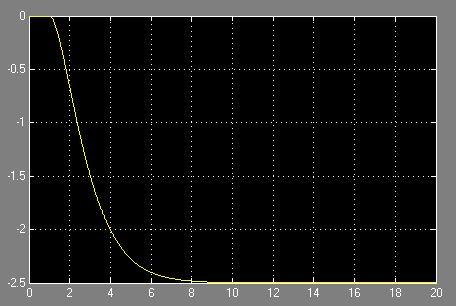
\includegraphics[width=0.70\textwidth]{pics/lowpassfilter}
	\caption{Prefilter response, Input step 0 to -2.5 at t=1 sec)}
	\label{3:fig:lowpassfilter}
\end{figure}

The filter damps the step response so it can be sent to the controller. This is that the controller is actually responding to, the user would not see this signal. The step response provided earlier is purely what the user sees in terms of input and output.

Switching the signal to a pulse (to examine response time to non-step input signals gives a far different response. The settling time would likely be almost fast enough to position itself reasonably from this waveform, but the filter attenuates the up and down impulses of the step waveform heavily, slowing the response. Initial conditions were unchanged for this pulse response test.

\begin{figure}[h!t]
	\centering
		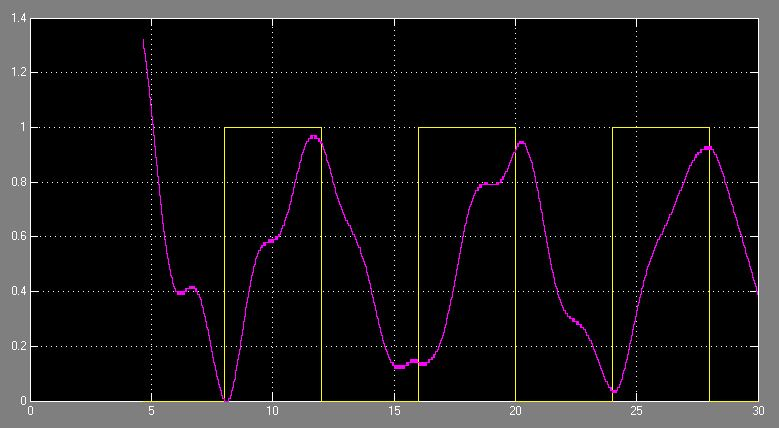
\includegraphics[width=0.70\textwidth]{pics/pulseresponse}
	\caption{Controller response to pulse input}
	\label{3:fig:pulseresponse}
\end{figure}
\FloatBarrier

Now the controller looks almost as if it is trying to follow a sinusoidal wave, but if we take a look at what the prefilter is doing to the signal, we see that it is not too far off from the reference signal it is receiving.

\begin{figure}[h!t]
	\centering
		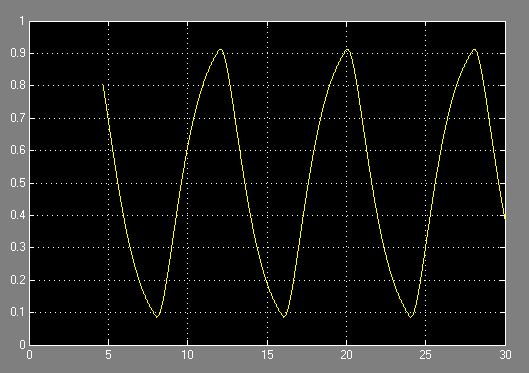
\includegraphics[width=0.70\textwidth]{pics/lowpasspulse}
	\caption{Filtered pulse input}
	\label{3:fig:lowpasspulse}
\end{figure}
\FloatBarrier

This is actually fairly close to what the controller is trying to produce. This prefilter does negatively impact the settling speed of the response, but it damps the controller's sudden inputs in the wrong direction which was considered more important given the sensitivity of the item being controlled.

